\documentclass[border=2mm]{standalone}
\usepackage{tikz}
\usepackage{tabu}

\begin{document}

\begin{tabu} to \textwidth{|c|c|}
\hline
\setlength\tabulinesep{2pt}
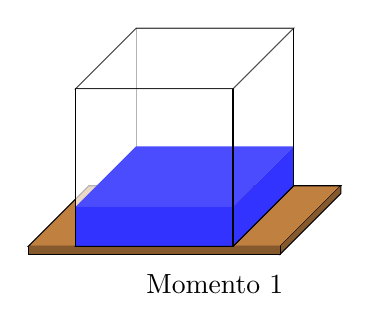
\begin{tikzpicture}[scale=2]



\draw [fill=brown] (-.3,0,0) -- (1.3,0,0) -- (1.3,0,1) -- (-.3,0,1) -- cycle;
\draw [fill=brown!70!black] (1.3,0,-0) -- (1.3,-.05,0) -- (1.3,-.05,1) -- (1.3,0,1);
\draw [fill=brown!70!black] (1.3,0,1) -- (1.3,-.05,1) -- (-.3,-.05,1) -- (-.3,0,1);



\draw (0,0,0) -- (1,0,0) -- (1,0,1) -- (0,0,1) -- cycle;

\draw (0,0,0) -- (0,1,0);
\draw [fill=white, opacity=.7] (0,1,0) -- (1,1,0) -- (1,1,1) -- (0,1,1) -- cycle;
\draw [fill=white, opacity=.7] (0,0,1) -- (1,0,1) -- (1,1,1) -- (0,1,1) -- cycle;

\fill [blue!70] (0,.25,0) -- (1,.25,0) -- (1,.25,1) -- (0,.25,1) -- cycle;
\fill [blue!80] (0,0,1) -- (1,0,1) -- (1,.25,1) -- (0,.25,1) -- cycle;
\fill [blue!80] (1,0,0) -- (1,0,1) -- (1,.25,1) -- (1,.25,0) -- cycle;

\draw (1,0,1) -- (1,1,1);
\draw (1,0,0) -- (1,1,0);
\draw (0,0,1) -- (0,1,1);
\draw (1,0,0) -- (1,0,1) -- (0,0,1);

\node[below] at (0.5,-.5) {Momento 1};
\end{tikzpicture}

& 

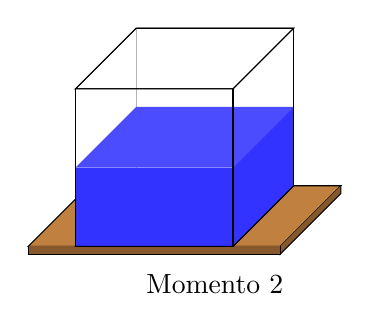
\begin{tikzpicture}[scale=2]

\draw [fill=brown] (-.3,0,0) -- (1.3,0,0) -- (1.3,0,1) -- (-.3,0,1) -- cycle;
\draw [fill=brown!70!black] (1.3,0,-0) -- (1.3,-.05,0) -- (1.3,-.05,1) -- (1.3,0,1);
\draw [fill=brown!70!black] (1.3,0,1) -- (1.3,-.05,1) -- (-.3,-.05,1) -- (-.3,0,1);



\draw (0,0,0) -- (1,0,0) -- (1,0,1) -- (0,0,1) -- cycle;

\draw (0,0,0) -- (0,1,0);
\draw [fill=white, opacity=.7] (0,1,0) -- (1,1,0) -- (1,1,1) -- (0,1,1) -- cycle;
\draw [fill=white, opacity=.7] (0,0,1) -- (1,0,1) -- (1,1,1) -- (0,1,1) -- cycle;

\fill [blue!70] (0,.5,0) -- (1,.5,0) -- (1,.5,1) -- (0,.5,1) -- cycle;
\fill [blue!80] (0,0,1) -- (1,0,1) -- (1,.5,1) -- (0,.5,1) -- cycle;
\fill [blue!80] (1,0,0) -- (1,0,1) -- (1,.5,1) -- (1,.5,0) -- cycle;

\draw (1,0,1) -- (1,1,1);
\draw (1,0,0) -- (1,1,0);
\draw (0,0,1) -- (0,1,1);
\draw (1,0,0) -- (1,0,1) -- (0,0,1);
\draw (0,1,0) -- (1,1,0) -- (1,1,1) -- (0,1,1) -- cycle;

\node[below] at (0.5,-.5) {Momento 2};
\end{tikzpicture} \\

\hline

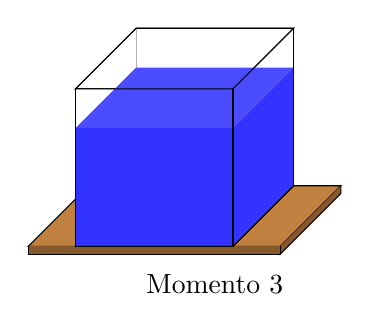
\begin{tikzpicture}[scale=2]

\draw [fill=brown] (-.3,0,0) -- (1.3,0,0) -- (1.3,0,1) -- (-.3,0,1) -- cycle;
\draw [fill=brown!70!black] (1.3,0,-0) -- (1.3,-.05,0) -- (1.3,-.05,1) -- (1.3,0,1);
\draw [fill=brown!70!black] (1.3,0,1) -- (1.3,-.05,1) -- (-.3,-.05,1) -- (-.3,0,1);



\draw (0,0,0) -- (1,0,0) -- (1,0,1) -- (0,0,1) -- cycle;

\draw (0,0,0) -- (0,1,0);
\draw [fill=white, opacity=.7] (0,1,0) -- (1,1,0) -- (1,1,1) -- (0,1,1) -- cycle;
\draw [fill=white, opacity=.7] (0,0,1) -- (1,0,1) -- (1,1,1) -- (0,1,1) -- cycle;

\fill [blue!70] (0,.75,0) -- (1,.75,0) -- (1,.75,1) -- (0,.75,1) -- cycle;
\fill [blue!80] (0,0,1) -- (1,0,1) -- (1,.75,1) -- (0,.75,1) -- cycle;
\fill [blue!80] (1,0,0) -- (1,0,1) -- (1,.75,1) -- (1,.75,0) -- cycle;

\draw (1,0,1) -- (1,1,1);
\draw (1,0,0) -- (1,1,0);
\draw (0,0,1) -- (0,1,1);
\draw (1,0,0) -- (1,0,1) -- (0,0,1);
\draw (0,1,0) -- (1,1,0) -- (1,1,1) -- (0,1,1) -- cycle;

\node[below] at (0.5,-.5) {Momento 3};
\end{tikzpicture}

& 
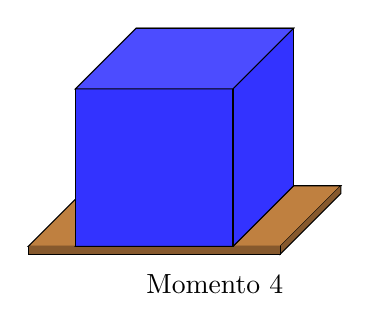
\begin{tikzpicture}[scale=2]

\draw [fill=brown] (-.3,0,0) -- (1.3,0,0) -- (1.3,0,1) -- (-.3,0,1) -- cycle;
\draw [fill=brown!70!black] (1.3,0,-0) -- (1.3,-.05,0) -- (1.3,-.05,1) -- (1.3,0,1);
\draw [fill=brown!70!black] (1.3,0,1) -- (1.3,-.05,1) -- (-.3,-.05,1) -- (-.3,0,1);



\draw (0,0,0) -- (1,0,0) -- (1,0,1) -- (0,0,1) -- cycle;

\draw (0,0,0) -- (0,1,0);
\draw [fill=white, opacity=.7] (0,1,0) -- (1,1,0) -- (1,1,1) -- (0,1,1) -- cycle;
\draw [fill=white, opacity=.7] (0,0,1) -- (1,0,1) -- (1,1,1) -- (0,1,1) -- cycle;


\fill [blue!70] (0,1,0) -- (1,1,0) -- (1,1,1) -- (0,1,1) -- cycle;
\fill [blue!80] (0,0,1) -- (1,0,1) -- (1,1,1) -- (0,1,1) -- cycle;
\fill [blue!80] (1,0,0) -- (1,0,1) -- (1,1,1) -- (1,1,0) -- cycle;

\draw (1,0,1) -- (1,1,1);
\draw (1,0,0) -- (1,1,0);
\draw (0,0,1) -- (0,1,1);
\draw (1,0,0) -- (1,0,1) -- (0,0,1);
\draw (0,1,0) -- (1,1,0) -- (1,1,1) -- (0,1,1) -- cycle;


\node[below] at (0.5,-.5) {Momento 4};
\end{tikzpicture} \\
\hline
\end{tabu}

\end{document}

